\documentclass{article}

% content/resources/templates/preamble.tex
\usepackage[margin=0.6in]{geometry}
\author{Milav Dabgar}
\usepackage{amsmath,amssymb,amsthm}
\usepackage{booktabs}
\usepackage{multirow}
\usepackage{xcolor}
\usepackage{tcolorbox}
\tcbuselibrary{breakable,skins}
\usepackage[colorlinks=true,linkcolor=blue]{hyperref}
\usepackage{titlesec}
\usepackage{enumitem}
\usepackage{tikz}
\usepackage{pgfplots}
\usepackage{circuitikz}
\usepackage[version=4]{mhchem}
\usepackage{longtable}
\usepackage{array}
\usepackage{float}
\usepackage{caption}
\usepackage{listings}

\lstset{
  basicstyle=\small\ttfamily,
  breaklines=true,
  breakatwhitespace=false,
  postbreak=\mbox{\textcolor{red}{$\hookrightarrow$}\space},
  float=false,
  numbers=left,
  numberstyle=\tiny\color{gray},
  numbersep=10pt,
  xleftmargin=2em,
  keywordstyle=\color{blue},
  commentstyle=\color{green!60!black},
  stringstyle=\color{purple},
  backgroundcolor=\color{gray!5},
  showstringspaces=false,
  tabsize=2,
  captionpos=b,
  keepspaces=true,
  columns=flexible
}

\pgfplotsset{compat=1.18}
\usetikzlibrary{shapes,arrows,positioning,calc,patterns,decorations.pathmorphing,decorations.markings,arrows.meta}

% Color scheme
\definecolor{headcolor}{RGB}{0,102,204}
\definecolor{keycolor}{RGB}{220,20,60}
\definecolor{solutioncolor}{RGB}{34,139,34}
\definecolor{mnemoniccolor}{RGB}{148,0,211}
\definecolor{codecolor}{RGB}{0,0,100}

% Spacing
\setlength{\parskip}{3pt}
\setlist[itemize]{nosep}
\setlist[enumerate]{nosep}

% Title formatting
\titleformat{\section}{\Large\bfseries\color{headcolor}}{\thesection}{1em}{}
\titleformat{\subsection}{\large\bfseries\color{headcolor}}{\thesubsection}{1em}{}

% Pandoc tightlist compatibility
\providecommand{\tightlist}{%
  \setlength{\itemsep}{0pt}\setlength{\parskip}{0pt}}

% Pandoc longtable compatibility
\newcounter{none}
\def\thenone{}


% content/resources/templates/english-boxes.tex

% Custom environments
\newtcolorbox{solutionbox}{
 breakable,
 enhanced,
 colback=solutioncolor!5!white,
 colframe=solutioncolor!75!black,
 fonttitle=\bfseries,
 title=Solution
}

\newtcolorbox{solutionboxnobreak}{
 colback=solutioncolor!5!white,
 colframe=solutioncolor!75!black,
 fonttitle=\bfseries,
 title=Solution
}

\newtcolorbox{keyformula}{
 breakable,
 enhanced,
 colback=keycolor!5!white,
 colframe=keycolor!75!black,
 fonttitle=\bfseries,
 title=Key Formula
}

\newtcolorbox{mnemonicboxenv}{
 breakable,
 enhanced,
 colback=mnemoniccolor!5!white,
 colframe=mnemoniccolor!75!black,
 fonttitle=\bfseries,
 title=Mnemonic
}

\newcommand{\mnemonicbox}[1]{%
  \begin{mnemonicboxenv}
    #1
  \end{mnemonicboxenv}
}


% Custom commands for GTU solutions
% This file defines semantic commands for consistent formatting

% Question command with automatic formatting
\newcommand{\question}[2]{%
  \section*{Question #1}%
  \textbf{#2}%
}

% OR question variant
\newcommand{\questionor}[2]{%
  \section*{Question #1 OR}%
  \textbf{#2}%
}

% Proper table environment with caption
\newenvironment{answertable}[1]{%
  \begin{table}[htbp]
  \centering
  \caption{#1}
}{%
  \end{table}
}

% Proper figure environment for diagrams
\newenvironment{answerdiagram}[1]{%
  \begin{figure}[htbp]
  \centering
  \caption{#1}
}{%
  \end{figure}
}

% Semantic markup for key terms
\newcommand{\keyword}[1]{\textbf{#1}}
\newcommand{\code}[1]{\texttt{#1}}
\newcommand{\classname}[1]{\texttt{#1}}
\newcommand{\methodname}[1]{\texttt{#1}}

% Proper quotation marks
\newcommand{\mnemonic}[1]{``#1''}


\title{Digital Communication (4341102) - Summer 2023 Solution}
\date{July 15, 2023}

\begin{document}
\maketitle

\questionmarks{1}{a}{3}
\textbf{Define signal and give its classification.}

\begin{solutionbox}
A \keyword{signal} is a physical quantity that varies with time, space, or any other independent variable and contains information.

\textbf{Classification of Signals:}

\begin{tabulary}{\linewidth}{L L}
\hline
\textbf{Classification Criteria} & \textbf{Types of Signals} \\
\hline
\textbf{Time Domain} & Continuous-time signals, Discrete-time signals \\
\textbf{Amplitude} & Analog signals, Digital signals \\
\textbf{Nature} & Deterministic signals, Random signals \\
\textbf{Symmetry} & Even signals, Odd signals \\
\textbf{Energy/Power} & Energy signals, Power signals \\
\hline
\end{tabulary}

\begin{mnemonicbox}
\textbf{Mnemonic:} "CADEN" (Continuous/Discrete, Analog/Digital, Deterministic/Random, Even/Odd, Energy/Power)
\end{mnemonicbox}
\end{solutionbox}

\questionmarks{1}{b}{4}
\textbf{Explain continuous and discrete time signals.}

\begin{solutionbox}
\begin{tabulary}{\linewidth}{L L}
\hline
\textbf{Continuous-time Signals} & \textbf{Discrete-time Signals} \\
\hline
Defined for all values of time & Defined only at specific time instants \\
Represented as $x(t)$ & Represented as $x[n]$ or $x(nT)$ \\
Example: Analog signals like sinusoidal wave & Example: Digital signals like sampled speech \\
Continuous curve on graph & Series of points on graph \\
Processing requires analog circuits & Processing can be done with digital processors \\
\hline
\end{tabulary}

\textbf{Diagram:}

\begin{center}
\begin{tikzpicture}[node distance=2.5cm, auto]
    \node [gtu block] (sig) {Signals};
    \node [gtu block, below left of=sig, xshift=-1cm] (cont) {Continuous-time};
    \node [gtu block, below right of=sig, xshift=1cm] (disc) {Discrete-time};
    \node [gtu block, below of=cont] (contex) {Defined for all $t$\\Example: $\sin(t)$};
    \node [gtu block, below of=disc] (discex) {Defined at specific instants $nT$\\Example: $\sin(nT)$};

    \path [gtu arrow] (sig) -- (cont);
    \path [gtu arrow] (sig) -- (disc);
    \path [gtu arrow] (cont) -- (contex);
    \path [gtu arrow] (disc) -- (discex);
\end{tikzpicture}
\end{center}

\begin{mnemonicbox}
\textbf{Mnemonic:} "CAD" - Continuous signals are Analog and Defined for all time; Discrete signals are digital and defined at specific points.
\end{mnemonicbox}
\end{solutionbox}

\questionmarks{1}{c}{7}
\textbf{Explain Unit Impulse and Unit Step function.}

\begin{solutionbox}
\begin{tabulary}{\linewidth}{L L}
\hline
\textbf{Unit Impulse Function ($\delta(t)$)} & \textbf{Unit Step Function ($u(t)$)} \\
\hline
Infinitely high at $t=0$, zero elsewhere & Value is 1 for $t \ge 0$, 0 for $t<0$ \\
Area under curve = 1 & Integral gives ramp function \\
Used to represent instantaneous events & Used to represent sudden transitions \\
Mathematical basis for LTI system analysis & Used for system response analysis \\
Laplace transform = 1 & Laplace transform = $1/s$ \\
\hline
\end{tabulary}

\textbf{Diagram:}

\begin{center}
\begin{tikzpicture}
    % Unit Impulse
    \begin{scope}[xshift=-4cm]
        \draw[->] (-2,0) -- (2,0) node[right] {$t$};
        \draw[->] (0,-0.5) -- (0,2.5);
        \draw[thick, ->] (0,0) -- (0,2) node[above] {$\delta(t)$};
        \node at (0.5, 1) {Area = 1};
        \node[below] at (0,-0.5) {Unit Impulse};
    \end{scope}

    % Unit Step
    \begin{scope}[xshift=4cm]
        \draw[->] (-2,0) -- (2,0) node[right] {$t$};
        \draw[->] (0,-0.5) -- (0,2.5) node[above] {$u(t)$};
        \draw[thick] (-2,0) -- (0,0);
        \draw[thick] (0,0) -- (0,1.5) -- (2,1.5);
        \node[left] at (0,1.5) {1};
        \node[below] at (0,-0.5) {Unit Step};
    \end{scope}
\end{tikzpicture}
\end{center}

\textbf{Properties:}
\begin{itemize}
    \item \textbf{Sampling property}: $\int f(t)\delta(t-t_0)dt = f(t_0)$
    \item \textbf{Unit step is integral of impulse}: $u(t) = \int_{-\infty}^{t} \delta(\tau)d\tau$
    \item \textbf{Impulse is derivative of unit step}: $\delta(t) = \frac{du(t)}{dt}$
\end{itemize}

\begin{mnemonicbox}
\textbf{Mnemonic:} "SHARP-FLAT" - Impulse is Sharp and momentary; Step is Flat and persistent.
\end{mnemonicbox}
\end{solutionbox}

\questionmarks{1}{c}{7}
\textbf{Explain block diagram of digital communication system.}

\begin{solutionbox}
\textbf{Block Diagram of Digital Communication System:}

\begin{center}
\begin{tikzpicture}[node distance=1.8cm, auto]
    \node [gtu block] (source) {Source};
    \node [gtu block, right of=source, node distance=2.5cm] (sec) {Source\\Encoder};
    \node [gtu block, right of=sec, node distance=2.5cm] (cec) {Channel\\Encoder};
    \node [gtu block, right of=cec, node distance=2.5cm] (mod) {Digital\\Modulator};
    
    \node [gtu block, below of=mod, node distance=2cm] (chan) {Channel};
    
    \node [gtu block, below of=chan, node distance=2cm] (demod) {Digital\\Demodulator};
    \node [gtu block, left of=demod, node distance=2.5cm] (cdec) {Channel\\Decoder};
    \node [gtu block, left of=cdec, node distance=2.5cm] (sdec) {Source\\Decoder};
    \node [gtu block, left of=sdec, node distance=2.5cm] (dest) {Destination};

    \path [gtu arrow] (source) -- (sec);
    \path [gtu arrow] (sec) -- (cec);
    \path [gtu arrow] (cec) -- (mod);
    \path [gtu arrow] (mod) -- (chan);
    \path [gtu arrow] (chan) -- (demod);
    \path [gtu arrow] (demod) -- (cdec);
    \path [gtu arrow] (cdec) -- (sdec);
    \path [gtu arrow] (sdec) -- (dest);
\end{tikzpicture}
\end{center}

\textbf{Explanation:}

\begin{tabulary}{\linewidth}{L L}
\hline
\textbf{Block} & \textbf{Function} \\
\hline
\textbf{Source} & Generates the message to be transmitted \\
\textbf{Source Encoder} & Converts message to digital form, removes redundancy \\
\textbf{Channel Encoder} & Adds controlled redundancy for error detection/correction \\
\textbf{Digital Modulator} & Maps digital bits to signals suitable for transmission \\
\textbf{Channel} & Physical medium through which signal travels \\
\textbf{Digital Demodulator} & Recovers digital data from received signal \\
\textbf{Channel Decoder} & Detects/corrects errors using added redundancy \\
\textbf{Source Decoder} & Reconstructs original message from received bits \\
\textbf{Destination} & Receives the transmitted message \\
\hline
\end{tabulary}

\begin{mnemonicbox}
\textbf{Mnemonic:} "SECDCSD" - "Seven Engineers Can Design Communication Systems Diligently"
\end{mnemonicbox}
\end{solutionbox}

\questionmarks{2}{a}{3}
\textbf{A signal has a bit rate of 8000 bit/second and a baud rate of 1000 baud. How many data elements are carried by each signal element?}

\begin{solutionbox}
Number of data elements (bits) per signal element:
\[ = \frac{\text{Bit rate}}{\text{Baud rate}} \]
\[ = \frac{8000 \text{ bits/second}}{1000 \text{ baud}} \]
\[ = 8 \text{ bits/signal element} \]

\textbf{Table:}

\begin{tabulary}{\linewidth}{L L L}
\hline
\textbf{Parameter} & \textbf{Value} & \textbf{Relation} \\
\hline
Bit rate & 8000 bits/sec & Given \\
Baud rate & 1000 baud & Given \\
Bits/signal & 8 bits & Bit rate $\div$ Baud rate \\
\hline
\end{tabulary}

\begin{mnemonicbox}
\textbf{Mnemonic:} "Bits Divided By Bauds" (BDBB)
\end{mnemonicbox}
\end{solutionbox}

\questionmarks{2}{b}{4}
\textbf{Explain Energy and power signals.}

\begin{solutionbox}
\begin{tabulary}{\linewidth}{L L}
\hline
\textbf{Energy Signals} & \textbf{Power Signals} \\
\hline
Finite total energy & Infinite total energy but finite average power \\
Zero average power & Non-zero average power \\
$E = \int |x(t)|^2 dt$ (finite) & $P = \lim_{T\to\infty} \frac{1}{2T} \int |x(t)|^2 dt$ (finite) \\
Examples: Pulse, Decaying exponential & Examples: Sine wave, Square wave \\
Localized in time & Exist for all time \\
\hline
\end{tabulary}

\textbf{Diagram:}

\begin{center}
\begin{tikzpicture}[node distance=2cm, auto]
    \node [gtu block] (sig) {Signals};
    \node [gtu block, below left of=sig, xshift=-1.5cm] (energy) {Energy Signals};
    \node [gtu block, below right of=sig, xshift=1.5cm] (power) {Power Signals};
    \node [gtu block, below of=energy, node distance=2.5cm] (eprop) {Finite Energy\\Zero Avg Power\\Ex: Pulse};
    \node [gtu block, below of=power, node distance=2.5cm] (pprop) {Infinite Energy\\Finite Avg Power\\Ex: Sine Wave};

    \path [gtu arrow] (sig) -- (energy);
    \path [gtu arrow] (sig) -- (power);
    \path [gtu arrow] (energy) -- (eprop);
    \path [gtu arrow] (power) -- (pprop);
\end{tikzpicture}
\end{center}

\begin{mnemonicbox}
\textbf{Mnemonic:} "FEZIL" - Finite Energy is Zero in Long-term; Power signals are Infinite in Length
\end{mnemonicbox}
\end{solutionbox}

\questionmarks{2}{c}{7}
\textbf{Explain the block diagram of FSK modulator and de-modulator with waveform.}

\begin{solutionbox}
\textbf{FSK Modulator and Demodulator:}

\begin{center}
\begin{tikzpicture}[node distance=2cm, auto]
    % Modulator
    \node [gtu block, minimum width=2.5cm] (input) {Digital Input};
    \node [gtu block, right of=input, node distance=4cm] (vco) {Voltage Controlled\\Oscillator (VCO)};
    \node [gtu block, right of=vco, node distance=4cm] (output) {FSK Output};
    
    \path [gtu arrow] (input) -- (vco);
    \path [gtu arrow] (vco) -- (output);
    
    \node [below of=vco, node distance=1.5cm, font=\bfseries] {Modulator};

    % Demodulator
    \node [gtu block, minimum width=2cm, below of=input, node distance=3.5cm] (fskinput) {FSK Input};
    
    \node [gtu block, right of=fskinput, node distance=3cm, yshift=1cm] (bpf1) {BPF 1\\($f_1$)};
    \node [gtu block, right of=fskinput, node distance=3cm, yshift=-1cm] (bpf2) {BPF 2\\($f_2$)};
    
    \node [gtu block, right of=bpf1, node distance=2.5cm] (env1) {Envelope\\Detector 1};
    \node [gtu block, right of=bpf2, node distance=2.5cm] (env2) {Envelope\\Detector 2};
    
    \node [gtu block, right of=env1, node distance=2.5cm, yshift=-1cm] (comp) {Comparator};
    \node [gtu block, right of=comp, node distance=2.5cm] (dout) {Digital Output};

    \path [gtu arrow] (fskinput) -- ++(1,0) |- (bpf1);
    \path [gtu arrow] (fskinput) -- ++(1,0) |- (bpf2);
    \path [gtu arrow] (bpf1) -- (env1);
    \path [gtu arrow] (bpf2) -- (env2);
    \path [gtu arrow] (env1) -| (comp);
    \path [gtu arrow] (env2) -| (comp);
    \path [gtu arrow] (comp) -- (dout);
    
    \node [below of=comp, node distance=2cm, font=\bfseries] {Demodulator};
\end{tikzpicture}
\end{center}

\textbf{Waveforms:}

\begin{center}
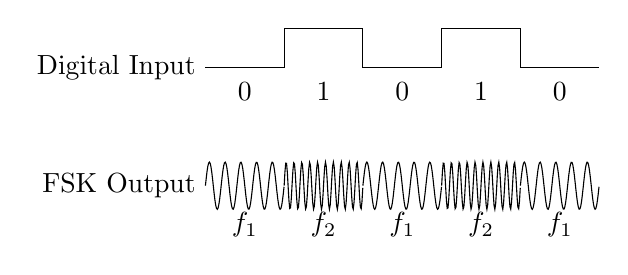
\begin{tikzpicture}
    % Digital Input
    \draw (0,4) node[left] {Digital Input};
    \draw (0,4) -- (1,4) -- (1,4.5) -- (2,4.5) -- (2,4) -- (3,4) -- (3,4.5) -- (4,4.5) -- (4,4) -- (5,4);
    \foreach \x/\val in {0.5/0, 1.5/1, 2.5/0, 3.5/1, 4.5/0}
        \node at (\x, 3.7) {\val};

    % FSK Output
    \draw (0,2.5) node[left] {FSK Output};
    % f1: low freq, f2: high freq
    \draw[samples=100, domain=0:1] plot (\x, {2.5 + 0.3*sin(1800*(\x - floor(\x)))});
    \draw[samples=100, domain=1:2] plot (\x, {2.5 + 0.3*sin(3600*(\x - floor(\x)))});
    \draw[samples=100, domain=2:3] plot (\x, {2.5 + 0.3*sin(1800*(\x - floor(\x)))});
    \draw[samples=100, domain=3:4] plot (\x, {2.5 + 0.3*sin(3600*(\x - floor(\x)))});
    \draw[samples=100, domain=4:5] plot (\x, {2.5 + 0.3*sin(1800*(\x - floor(\x)))});
    
    \foreach \x/\val in {0.5/$f_1$, 1.5/$f_2$, 2.5/$f_1$, 3.5/$f_2$, 4.5/$f_1$}
        \node at (\x, 2) {\val};
\end{tikzpicture}
\end{center}

\textbf{Key Principles:}
\begin{itemize}
    \item \textbf{Bit 0}: Transmitted as frequency $f_1$
    \item \textbf{Bit 1}: Transmitted as frequency $f_2$
    \item \textbf{Demodulation}: Uses bandpass filters to separate frequencies
    \item \textbf{Detection}: Envelope detectors recover the digital signal
\end{itemize}

\begin{mnemonicbox}
\textbf{Mnemonic:} "FIST" - Frequency Is Shifted for Transmission
\end{mnemonicbox}
\end{solutionbox}

\questionmarks{2}{a}{3}
\textbf{A signal carries 4 bit/signal elements. If 1000 signal elements sent per second. Find the bit rate.}

\begin{solutionbox}
Bit rate = Number of bits per signal element $\times$ Signal elements per second \\
Bit rate = 4 bits/signal element $\times$ 1000 signal elements/second \\
Bit rate = 4000 bits/second

\textbf{Table:}

\begin{tabulary}{\linewidth}{L L L}
\hline
\textbf{Parameter} & \textbf{Value} & \textbf{Relation} \\
\hline
Bits per symbol & 4 & Given \\
Symbol rate & 1000 symbols/sec & Given \\
Bit rate & 4000 bits/sec & Bits/symbol $\times$ Symbol rate \\
\hline
\end{tabulary}

\begin{mnemonicbox}
\textbf{Mnemonic:} "BBS" - Bit rate equals Bits per symbol times Symbol rate
\end{mnemonicbox}
\end{solutionbox}

\questionmarks{2}{b}{4}
\textbf{Explain Even and Odd signals.}

\begin{solutionbox}
\begin{tabulary}{\linewidth}{L L}
\hline
\textbf{Even Signals} & \textbf{Odd Signals} \\
\hline
Symmetric around y-axis & Anti-symmetric around y-axis \\
$x(-t) = x(t)$ & $x(-t) = -x(t)$ \\
Example: $\cos(t)$ & Example: $\sin(t)$ \\
Fourier transform is real & Fourier transform is imaginary \\
Sum of even signals is even & Sum of odd signals is odd \\
\hline
\end{tabulary}

\textbf{Diagram:}

\begin{center}
\begin{tikzpicture}
    % Even Signal
    \begin{scope}[xshift=-4cm]
        \draw[->] (-2.5,0) -- (2.5,0) node[right] {$t$};
        \draw[->] (0,-1.5) -- (0,2) node[above] {$x(t)$ (Even)};
        \draw[thick, domain=-2:2, samples=50] plot (\x, {cos(90*\x)});
        \node[above] at (0,2) {};
    \end{scope}

    % Odd Signal
    \begin{scope}[xshift=4cm]
        \draw[->] (-2.5,0) -- (2.5,0) node[right] {$t$};
        \draw[->] (0,-1.5) -- (0,2) node[above] {$x(t)$ (Odd)};
        \draw[thick, domain=-2:2, samples=50] plot (\x, {sin(90*\x)});
    \end{scope}
\end{tikzpicture}
\end{center}

\textbf{Properties:}
\begin{itemize}
    \item Any signal can be expressed as sum of even and odd components
    \item Even component: $x_e(t) = [x(t) + x(-t)]/2$
    \item Odd component: $x_o(t) = [x(t) - x(-t)]/2$
\end{itemize}

\begin{mnemonicbox}
\textbf{Mnemonic:} "SAME-FLIP" - Even signals are the SAME when flipped; Odd signals FLIP their sign.
\end{mnemonicbox}
\end{solutionbox}

\questionmarks{2}{c}{7}
\textbf{Explain the block diagram of QPSK modulator and de-modulator with constellation diagram.}

\begin{solutionbox}
\textbf{QPSK Modulator and Demodulator:}

\begin{center}
\begin{tikzpicture}[node distance=2cm, auto]
    % Modulator
    \node [gtu block] (input) {Binary Input};
    \node [gtu block, right of=input, node distance=2.5cm] (sp) {S/P\\Converter};
    
    \node [gtu block, right of=sp, node distance=2.5cm, yshift=1cm] (mult1) {Multiplier};
    \node [gtu block, right of=sp, node distance=2.5cm, yshift=-1cm] (mult2) {Multiplier};
    
    \node [left of=mult1, node distance=1.2cm, above] {Even Bits};
    \node [left of=mult2, node distance=1.2cm, below] {Odd Bits};
    
    \node [above of=mult1, node distance=1cm] (cos) {$\cos(2\pi ft)$};
    \node [below of=mult2, node distance=1cm] (sin) {$\sin(2\pi ft)$};
    
    \node [gtu block, right of=mult1, node distance=2cm, yshift=-1cm] (sum) {Summer};
    \node [gtu block, right of=sum, node distance=2cm] (out) {QPSK Output};

    \path [gtu arrow] (input) -- (sp);
    \path [gtu arrow] (sp) |- (mult1);
    \path [gtu arrow] (sp) |- (mult2);
    \path [gtu arrow] (cos) -- (mult1);
    \path [gtu arrow] (sin) -- (mult2);
    \path [gtu arrow] (mult1) -| (sum);
    \path [gtu arrow] (mult2) -| (sum);
    \path [gtu arrow] (sum) -- (out);
\end{tikzpicture}
\end{center}

\textbf{Constellation Diagram:}

\begin{center}
\begin{tikzpicture}
    \draw[->] (-2,0) -- (2,0) node[right] {$I$};
    \draw[->] (0,-2) -- (0,2) node[above] {$Q$};
    
    \node[circle, fill, inner sep=1.5pt, label={45:00}] at (1,1) {};
    \node[circle, fill, inner sep=1.5pt, label={135:01}] at (-1,1) {};
    \node[circle, fill, inner sep=1.5pt, label={225:11}] at (-1,-1) {};
    \node[circle, fill, inner sep=1.5pt, label={315:10}] at (1,-1) {};
    
    \draw[dashed] (1,0) -- (1,1) -- (0,1);
    \draw[dashed] (-1,0) -- (-1,1) -- (0,1);
    \draw[dashed] (-1,0) -- (-1,-1) -- (0,-1);
    \draw[dashed] (1,0) -- (1,-1) -- (0,-1);
\end{tikzpicture}
\end{center}

\textbf{Key Characteristics:}
\begin{itemize}
    \item \textbf{Input}: 2 bits determine each symbol
    \item \textbf{Phases}: 4 phases ($0^\circ, 90^\circ, 180^\circ, 270^\circ$)
    \item \textbf{Bits to phases}: 00: $45^\circ$, 01: $135^\circ$, 11: $225^\circ$, 10: $315^\circ$
    \item \textbf{Bandwidth efficiency}: 2 bits per symbol
\end{itemize}

\begin{mnemonicbox}
\textbf{Mnemonic:} "QUADrature" - 4 phases for 4 possible 2-bit combinations
\end{mnemonicbox}
\end{solutionbox}

\questionmarks{3}{a}{3}
\textbf{Explain the working of ASK modulator with block diagram and output waveforms.}

\begin{solutionbox}
\textbf{ASK Modulator Block Diagram:}

\begin{center}
\begin{tikzpicture}[node distance=2.5cm, auto]
    \node [gtu block] (input) {Digital Input};
    \node [gtu block, right of=input] (mult) {Multiplier};
    \node [gtu block, below of=mult] (gen) {Carrier Generator\\$\sin(2\pi ft)$};
    \node [gtu block, right of=mult] (out) {ASK Output};

    \path [gtu arrow] (input) -- (mult);
    \path [gtu arrow] (gen) -- (mult);
    \path [gtu arrow] (mult) -- (out);
\end{tikzpicture}
\end{center}

\textbf{Waveforms:}

\begin{center}
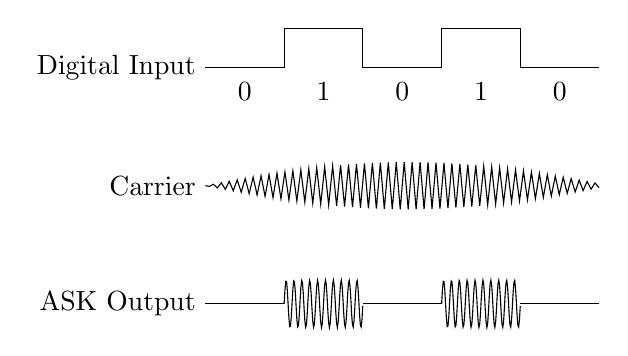
\begin{tikzpicture}
    % Digital Input
    \draw (0,4) node[left] {Digital Input};
    \draw (0,4) -- (1,4) -- (1,4.5) -- (2,4.5) -- (2,4) -- (3,4) -- (3,4.5) -- (4,4.5) -- (4,4) -- (5,4);
    \foreach \x/\val in {0.5/0, 1.5/1, 2.5/0, 3.5/1, 4.5/0}
        \node at (\x, 3.7) {\val};

    % Carrier
    \draw (0,2.5) node[left] {Carrier};
    \draw[samples=100, domain=0:5] plot (\x, {2.5 + 0.3*sin(3600*(\x - floor(\x)))});

    % ASK Output
    \draw (0,1) node[left] {ASK Output};
    % 0: flat, 1: carrier
    \draw[samples=100, domain=0:1] plot (\x, {1});
    \draw[samples=100, domain=1:2] plot (\x, {1 + 0.3*sin(3600*(\x - floor(\x)))});
    \draw[samples=100, domain=2:3] plot (\x, {1});
    \draw[samples=100, domain=3:4] plot (\x, {1 + 0.3*sin(3600*(\x - floor(\x)))});
    \draw[samples=100, domain=4:5] plot (\x, {1});
\end{tikzpicture}
\end{center}

\textbf{Working Principle:}
\begin{itemize}
    \item Digital 1: Carrier signal is transmitted
    \item Digital 0: No signal (or low amplitude) is transmitted
    \item Output amplitude varies with input digital signal
\end{itemize}

\begin{mnemonicbox}
\textbf{Mnemonic:} "ASKY" - Amplitude Switches the Carrier? Yes!
\end{mnemonicbox}
\end{solutionbox}

\questionmarks{3}{b}{4}
\textbf{Draw the constellation diagram of 8-PSK and 16-QAM.}

\begin{solutionbox}
\textbf{8-PSK Constellation Diagram:}

\begin{center}
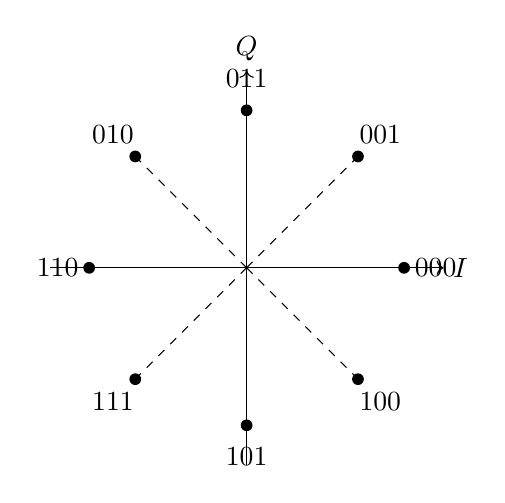
\begin{tikzpicture}
    \draw[->] (-2.5,0) -- (2.5,0) node[right] {$I$};
    \draw[->] (0,-2.5) -- (0,2.5) node[above] {$Q$};
    
    \foreach \ang/\lbl in {0/000, 45/001, 90/011, 135/010, 180/110, 225/111, 270/101, 315/100} {
        \node[circle, fill, inner sep=1.5pt] at (\ang:2) {};
        \node at (\ang:2.4) {\lbl};
        \draw[dashed] (0,0) -- (\ang:2);
    }
\end{tikzpicture}
\end{center}

\textbf{16-QAM Constellation Diagram:}

\begin{center}
\begin{tikzpicture}
    \draw[->] (-3,0) -- (3,0) node[right] {$I$};
    \draw[->] (0,-3) -- (0,3) node[above] {$Q$};
    
    \foreach \x in {-1.5, -0.5, 0.5, 1.5}
        \foreach \y in {-1.5, -0.5, 0.5, 1.5}
            \node[circle, fill, inner sep=1.5pt] at (\x,\y) {};
            
    \node at (0, -3.5) {16 points with varying Amplitude and Phase};
\end{tikzpicture}
\end{center}

\begin{mnemonicbox}
\textbf{Mnemonic:} "P-Phase Q-Quantity" - PSK varies Phase only; QAM varies both amplitude (Quantity) and phase
\end{mnemonicbox}
\end{solutionbox}

\questionmarks{3}{c}{7}
\textbf{Draw the ASK and FSK modulation waveform for the sequence of 1100101101.}

\begin{solutionbox}
\textbf{Modulation Waveforms:}

\begin{center}
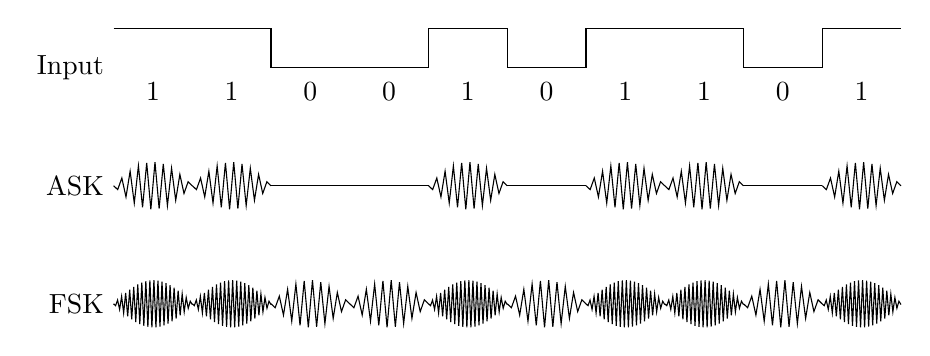
\begin{tikzpicture}
    % Sequence: 1 1 0 0 1 0 1 1 0 1
    % Binary Input
    \draw (0,4) node[left] {Input};
    \draw (0,4.5) -- (2,4.5) -- (2,4) -- (4,4) -- (4,4.5) -- (5,4.5) -- (5,4) -- (6,4) -- (6,4.5) -- (8,4.5) -- (8,4) -- (9,4) -- (9,4.5) -- (10,4.5);
    \foreach \x/\val in {0.5/1, 1.5/1, 2.5/0, 3.5/0, 4.5/1, 5.5/0, 6.5/1, 7.5/1, 8.5/0, 9.5/1}
        \node at (\x, 3.7) {\val};

    % ASK Output
    \draw (0,2.5) node[left] {ASK};
    \foreach \x/\val in {0/1, 1/1, 2/0, 3/0, 4/1, 5/0, 6/1, 7/1, 8/0, 9/1} {
        \ifnum\val=1
            \draw[samples=20, domain=\x:\x+1, variable=\u] plot[variable=\u] (\u, {2.5 + 0.3*sin(3600*(\u - floor(\u)))});
        \else
            \draw (\x,2.5) -- (\x+1,2.5);
        \fi
    }

    % FSK Output
    \draw (0,1) node[left] {FSK};
    \foreach \x/\val in {0/1, 1/1, 2/0, 3/0, 4/1, 5/0, 6/1, 7/1, 8/0, 9/1} {
        \ifnum\val=1
            % f2 (high freq) for 1
            \draw[samples=40, domain=\x:\x+1, variable=\u] plot[variable=\u] (\u, {1 + 0.3*sin(7200*(\u - floor(\u)))});
        \else
            % f1 (low freq) for 0
            \draw[samples=20, domain=\x:\x+1, variable=\u] plot[variable=\u] (\u, {1 + 0.3*sin(3600*(\u - floor(\u)))});
        \fi
    }
\end{tikzpicture}
\end{center}

\begin{tabulary}{\linewidth}{L L L L}
\hline
\textbf{Modulation} & \textbf{Bit 0} & \textbf{Bit 1} & \textbf{Parameter Varied} \\
\hline
ASK & Zero or low amplitude & High amplitude & Amplitude \\
FSK & Frequency $f_1$ & Frequency $f_2$ & Frequency \\
\hline
\end{tabulary}

\begin{mnemonicbox}
\textbf{Mnemonic:} "AFRO" - Amplitude For 1, Remove for 0 (ASK); Frequency Rises for 1, Off-peak for 0 (FSK)
\end{mnemonicbox}
\end{solutionbox}

\questionmarks{3}{a}{3}
\textbf{Explain the working of PSK modulator with block diagram and output waveforms.}

\begin{solutionbox}
\textbf{PSK Modulator Block Diagram:}

\begin{center}
\begin{tikzpicture}[node distance=2.5cm, auto]
    \node [gtu block] (input) {Digital Input};
    \node [gtu block, right of=input] (polar) {Polar Converter\\$0\to-1, 1\to+1$};
    \node [gtu block, right of=polar] (mult) {Multiplier};
    \node [gtu block, below of=mult] (gen) {Carrier Generator\\$\sin(2\pi ft)$};
    \node [gtu block, right of=mult] (out) {PSK Output};

    \path [gtu arrow] (input) -- (polar);
    \path [gtu arrow] (polar) -- (mult);
    \path [gtu arrow] (gen) -- (mult);
    \path [gtu arrow] (mult) -- (out);
\end{tikzpicture}
\end{center}

\textbf{Waveforms:}

\begin{center}
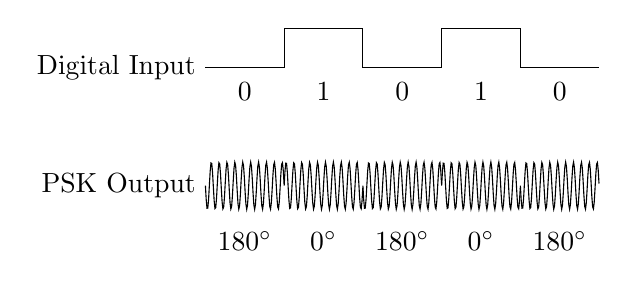
\begin{tikzpicture}
    % Digital Input
    \draw (0,4) node[left] {Digital Input};
    \draw (0,4) -- (1,4) -- (1,4.5) -- (2,4.5) -- (2,4) -- (3,4) -- (3,4.5) -- (4,4.5) -- (4,4) -- (5,4);
    \foreach \x/\val in {0.5/0, 1.5/1, 2.5/0, 3.5/1, 4.5/0}
        \node at (\x, 3.7) {\val};

    % PSK Output
    \draw (0,2.5) node[left] {PSK Output};
    % 0 -> 180 deg (inverted sine), 1 -> 0 deg (sine)
    \draw[samples=100, domain=0:1] plot (\x, {2.5 - 0.3*sin(3600*(\x - floor(\x)))});
    \draw[samples=100, domain=1:2] plot (\x, {2.5 + 0.3*sin(3600*(\x - floor(\x)))});
    \draw[samples=100, domain=2:3] plot (\x, {2.5 - 0.3*sin(3600*(\x - floor(\x)))});
    \draw[samples=100, domain=3:4] plot (\x, {2.5 + 0.3*sin(3600*(\x - floor(\x)))});
    \draw[samples=100, domain=4:5] plot (\x, {2.5 - 0.3*sin(3600*(\x - floor(\x)))});
    
    \foreach \x/\val in {0.5/$180^\circ$, 1.5/$0^\circ$, 2.5/$180^\circ$, 3.5/$0^\circ$, 4.5/$180^\circ$}
        \node at (\x, 1.8) {\val};
\end{tikzpicture}
\end{center}

\textbf{Working Principle:}
\begin{itemize}
    \item Digital 1: Carrier signal with $0^\circ$ phase
    \item Digital 0: Carrier signal with $180^\circ$ phase (inverted)
    \item Amplitude remains constant, only phase changes
\end{itemize}

\begin{mnemonicbox}
\textbf{Mnemonic:} "PSKIT" - Phase Shift Keeps Information True
\end{mnemonicbox}
\end{solutionbox}

\questionmarks{3}{b}{4}
\textbf{Draw the MSK modulation waveform for the sequence of 1101001101.}

\begin{solutionbox}
\textbf{MSK Modulation Waveform:}

\begin{center}
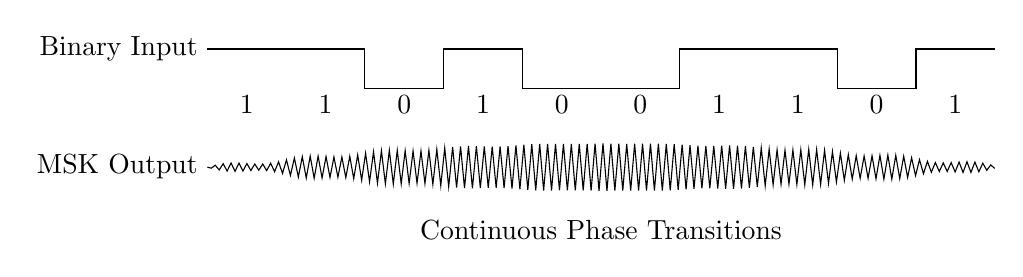
\begin{tikzpicture}
    % Input: 1 1 0 1 0 0 1 1 0 1
    \draw (0,2.5) node[left] {Binary Input};
    \draw (0,2.5) -- (2,2.5) -- (2,2) -- (3,2) -- (3,2.5) -- (4,2.5) -- (4,2) -- (6,2) -- (6,2.5) -- (8,2.5) -- (8,2) -- (9,2) -- (9,2.5) -- (10,2.5);
    \foreach \x/\val in {0.5/1, 1.5/1, 2.5/0, 3.5/1, 4.5/0, 5.5/0, 6.5/1, 7.5/1, 8.5/0, 9.5/1}
        \node at (\x, 1.8) {\val};

    \draw (0,1) node[left] {MSK Output};
    % Simplified representation of MSK (continuous phase, freq shift)
    % Not mathematically exact but visually representative of smoothness
    \draw[samples=200, domain=0:10] plot (\x, {1 + 0.3*sin((3600*(\x - floor(\x)) + 5*sin(360*\x)))}); 
    
    \node at (5, 0.2) {Continuous Phase Transitions};
\end{tikzpicture}
\end{center}

\textbf{Characteristics of MSK:}
\begin{itemize}
    \item Continuous phase transitions (no phase jumps)
    \item Frequency shifts between $f_1$ and $f_2$
    \item Minimum frequency separation: $\Delta f = 1/(2T)$
    \item Smoother transitions than FSK
\end{itemize}

\begin{tabulary}{\linewidth}{L L}
\hline
\textbf{Feature} & \textbf{MSK Characteristic} \\
\hline
Phase continuity & Continuous, no abrupt changes \\
Frequency deviation & Minimum possible (1/2T) \\
Spectral efficiency & Better than conventional FSK \\
Bandwidth & 1.5 times bit rate \\
\hline
\end{tabulary}

\begin{mnemonicbox}
\textbf{Mnemonic:} "MINIMUM SMOOTH" - MSK uses Minimum frequency separation with Smooth transitions
\end{mnemonicbox}
\end{solutionbox}

\questionmarks{3}{c}{7}
\textbf{Draw BPSK and QPSK modulation waveform for 1100101011.}

\begin{solutionbox}
\textbf{BPSK and QPSK Modulation Waveforms:}

\begin{center}
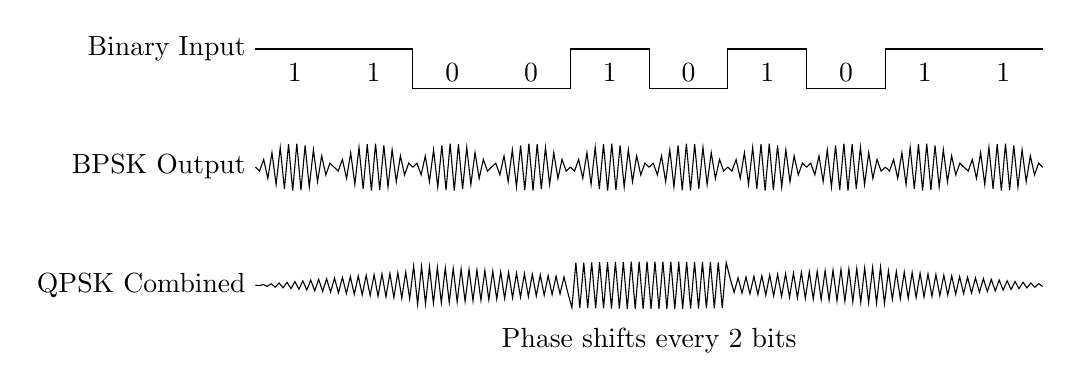
\begin{tikzpicture}
    % Input: 1 1 0 0 1 0 1 0 1 1
    \draw (0,5.5) node[left] {Binary Input};
    \draw (0,5.5) -- (2,5.5) -- (2,5) -- (4,5) -- (4,5.5) -- (5,5.5) -- (5,5) -- (6,5) -- (6,5.5) -- (7,5.5) -- (7,5) -- (8,5) -- (8,5.5) -- (10,5.5);
    \foreach \x/\val in {0.5/1, 1.5/1, 2.5/0, 3.5/0, 4.5/1, 5.5/0, 6.5/1, 7.5/0, 8.5/1, 9.5/1}
        \node at (\x, 5.2) {\val};

    % BPSK Output
    \draw (0,4) node[left] {BPSK Output};
    \foreach \x/\val in {0/1, 1/1, 2/0, 3/0, 4/1, 5/0, 6/1, 7/0, 8/1, 9/1} {
        \ifnum\val=1
            \draw[samples=20, domain=\x:\x+1] plot[variable=\u] (\u, {4 + 0.3*sin(3600*(\u - floor(\u)))});
        \else
            \draw[samples=20, domain=\x:\x+1] plot[variable=\u] (\u, {4 - 0.3*sin(3600*(\u - floor(\u)))});
        \fi
    }

    % QPSK - Simplified
    % I channel (odd bits: 1 1 1 1 1) -> 1 0 1 1 1 (based on index 1,3,5...) -> 1, 0, 1, 1, 1
    % Q channel (even bits: 1 0 0 0 1) -> 1, 0, 0, 0, 1
    
    \draw (0,2.5) node[left] {QPSK Combined};
    \draw[samples=200, domain=0:10] plot (\x, {2.5 + 0.3*sin((3600*(\x - floor(\x)) + 90*(int(\x/2))))});
    
    \node at (5, 1.8) {Phase shifts every 2 bits};

\end{tikzpicture}
\end{center}

\textbf{Key Differences:}
\begin{itemize}
    \item \textbf{BPSK}: 1 bit per symbol, 2 phases ($0^\circ$ and $180^\circ$)
    \item \textbf{QPSK}: 2 bits per symbol, 4 phases ($45^\circ, 135^\circ, 225^\circ, 315^\circ$)
    \item \textbf{QPSK Pairs}: 00, 01, 10, 11 map to different phases
\end{itemize}

\begin{tabulary}{\linewidth}{L L L L}
\hline
\textbf{Modulation} & \textbf{Bits/Symbol} & \textbf{Num Phases} & \textbf{BW Efficiency} \\
\hline
BPSK & 1 & 2 & 1 bit/Hz \\
QPSK & 2 & 4 & 2 bits/Hz \\
\hline
\end{tabulary}

\begin{mnemonicbox}
\textbf{Mnemonic:} "ONE-TWO" - ONE bit for BPSK, TWO bits for QPSK
\end{mnemonicbox}
\end{solutionbox}

\questionmarks{4}{a}{3}
\textbf{Encode the data using Huffman code for below probability sequence. P = \{ 0.4, 0.2, 0.2, 0.1, 0.1\}}

\begin{solutionbox}
\textbf{Huffman Coding Process:}

\begin{tabulary}{\linewidth}{L L L}
\hline
\textbf{Symbol} & \textbf{Probability} & \textbf{Huffman Code} \\
\hline
A & 0.4 & 0 \\
B & 0.2 & 10 \\
C & 0.2 & 11 \\
D & 0.1 & 110 \\
E & 0.1 & 111 \\
\hline
\end{tabulary}

\textbf{Huffman Tree:}

\begin{center}
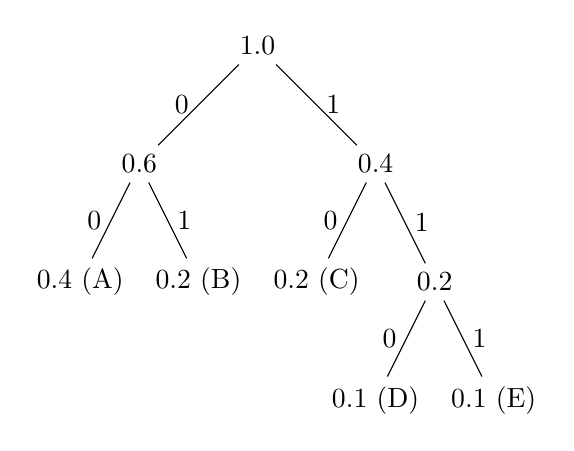
\begin{tikzpicture}[level distance=1.5cm,
  level 1/.style={sibling distance=3cm},
  level 2/.style={sibling distance=1.5cm},
  level 3/.style={sibling distance=1.5cm}]
  \node {1.0}
    child {node {0.6}
      child {node {0.4 (A)} edge from parent node[left] {0}}
      child {node {0.2 (B)} edge from parent node[right] {1}}
    edge from parent node[left] {0}}
    child {node {0.4}
      child {node {0.2 (C)} edge from parent node[left] {0}}
      child {node {0.2}
        child {node {0.1 (D)} edge from parent node[left] {0}}
        child {node {0.1 (E)} edge from parent node[right] {1}}
      edge from parent node[right] {1}}
    edge from parent node[right] {1}};
\end{tikzpicture}
\end{center}

\begin{mnemonicbox}
\textbf{Mnemonic:} "Higher Probability Means Shorter Code"
\end{mnemonicbox}
\end{solutionbox}

\questionmarks{4}{b}{4}
\textbf{Define Probability and Entropy.}

\begin{solutionbox}
\begin{tabulary}{\linewidth}{L L L L}
\hline
\textbf{Concept} & \textbf{Definition} & \textbf{Formula} & \textbf{Significance} \\
\hline
\textbf{Probability} & Measure of likelihood of an event occurring & $P(A) = \frac{\text{Favorable outcomes}}{\text{Total outcomes}}$ & Used to model uncertainty in communication \\
\textbf{Entropy} & Measure of uncertainty or randomness in a system & $H(X) = -\sum P(x_i) \log_2 P(x_i)$ & Indicates average information content \\
\hline
\end{tabulary}

\textbf{Key Characteristics:}
\begin{itemize}
    \item \textbf{Probability Range}: $0 \le P(A) \le 1$
    \item \textbf{Entropy Units}: Bits (using $\log_2$)
    \item \textbf{Maximum Entropy}: When all events are equally likely
    \item \textbf{Minimum Entropy}: When outcome is certain (probability = 1)
\end{itemize}

\begin{mnemonicbox}
\textbf{Mnemonic:} "PURE" - Probability Underpins Randomness Estimation
\end{mnemonicbox}
\end{solutionbox}

\questionmarks{4}{c}{7}
\textbf{Explain CDMA technique in detail.}

\begin{solutionbox}
\textbf{CDMA (Code Division Multiple Access):}

\begin{center}
\begin{tikzpicture}[node distance=2.5cm, auto]
    \node [gtu block] (data) {User Data};
    \node [gtu block, right of=data] (spread) {Spreading\\(Unique Code)};
    \node [gtu block, right of=spread] (mod) {Modulation};
    \node [gtu block, right of=mod] (trans) {Transmission};
    \node [gtu block, right of=trans] (rec) {Reception};
    
    \node [gtu block, below of=rec] (demod) {Demodulation};
    \node [gtu block, left of=demod] (despread) {Despreading\\(Matching Code)};
    \node [gtu block, left of=despread] (out) {Original Data};

    \path [gtu arrow] (data) -- (spread);
    \path [gtu arrow] (spread) -- (mod);
    \path [gtu arrow] (mod) -- (trans);
    \path [gtu arrow] (trans) -- (rec);
    \path [gtu arrow] (rec) -- (demod);
    \path [gtu arrow] (demod) -- (despread);
    \path [gtu arrow] (despread) -- (out);
\end{tikzpicture}
\end{center}

\textbf{Table of CDMA Characteristics:}

\begin{tabulary}{\linewidth}{L L}
\hline
\textbf{Feature} & \textbf{Description} \\
\hline
\textbf{Access Method} & Multiple users share same frequency and time \\
\textbf{Separation} & Users distinguished by unique spreading codes \\
\textbf{Spreading Codes} & Orthogonal or pseudo-orthogonal sequences \\
\textbf{Processing Gain} & Ratio of spread bandwidth to original bandwidth \\
\textbf{Multiple Access} & Uses code space rather than frequency or time division \\
\textbf{Interference Rejection} & Inherent ability to reject narrowband interference \\
\hline
\end{tabulary}

\textbf{Key Advantages:}
\begin{itemize}
    \item \textbf{Capacity}: Higher than FDMA/TDMA in many scenarios
    \item \textbf{Security}: Inherent encryption through spreading codes
    \item \textbf{Multipath Rejection}: Rake receivers can combine multipath components
    \item \textbf{Soft Handoff}: Mobile can communicate with multiple base stations
\end{itemize}

\begin{mnemonicbox}
\textbf{Mnemonic:} "CODES" - Capacity Optimized with Direct-sequence Encoding Schemes
\end{mnemonicbox}
\end{solutionbox}

\questionmarks{4}{a}{3}
\textbf{Encode the data using Shanon Fano code for below probability sequence. P = \{ 0.5, 0.25, 0.125, 0.125\}}

\begin{solutionbox}
\textbf{Shannon-Fano Coding Process:}

\begin{tabulary}{\linewidth}{L L L}
\hline
\textbf{Symbol} & \textbf{Probability} & \textbf{Shannon-Fano Code} \\
\hline
A & 0.5 & 0 \\
B & 0.25 & 10 \\
C & 0.125 & 110 \\
D & 0.125 & 111 \\
\hline
\end{tabulary}

\textbf{Shannon-Fano Tree:}

\begin{center}
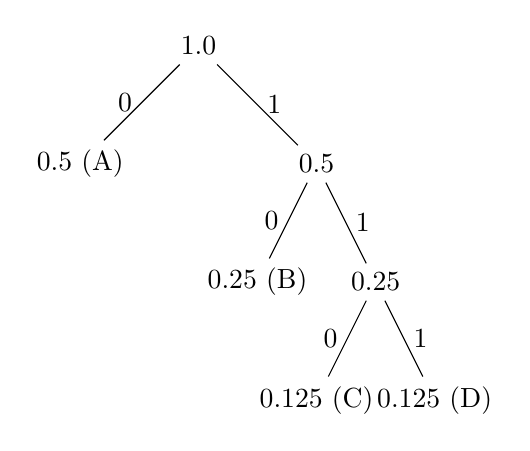
\begin{tikzpicture}[level distance=1.5cm,
  level 1/.style={sibling distance=3cm},
  level 2/.style={sibling distance=1.5cm},
  level 3/.style={sibling distance=1.5cm}]
  \node {1.0}
    child {node {0.5 (A)} edge from parent node[left] {0}}
    child {node {0.5}
      child {node {0.25 (B)} edge from parent node[left] {0}}
      child {node {0.25}
        child {node {0.125 (C)} edge from parent node[left] {0}}
        child {node {0.125 (D)} edge from parent node[right] {1}}
      edge from parent node[right] {1}}
    edge from parent node[right] {1}};
\end{tikzpicture}
\end{center}

\begin{mnemonicbox}
\textbf{Mnemonic:} "Split For Optimum" - Shannon-Fano splits groups for optimum coding
\end{mnemonicbox}
\end{solutionbox}

\questionmarks{4}{b}{4}
\textbf{Define Information and Channel Capacity.}

\begin{solutionbox}
\begin{tabulary}{\linewidth}{L L L L}
\hline
\textbf{Concept} & \textbf{Definition} & \textbf{Formula} & \textbf{Significance} \\
\hline
\textbf{Information} & Measure of reduction in uncertainty & $I(x) = -\log_2 P(x)$ & Less probable events carry more information \\
\textbf{Channel Capacity} & Maximum rate at which information can be transmitted with arbitrarily small error & $C = B \log_2(1 + S/N)$ & Fundamental limit of reliable communication \\
\hline
\end{tabulary}

\textbf{Key Points:}
\begin{itemize}
    \item \textbf{Information Units}: Bits (using $\log_2$)
    \item \textbf{Channel Capacity Units}: Bits per second
    \item \textbf{Factors Affecting Capacity}:
    \begin{itemize}
        \item Bandwidth (B)
        \item Signal-to-Noise Ratio (S/N)
    \end{itemize}
\end{itemize}

\begin{mnemonicbox}
\textbf{Mnemonic:} "INCHES" - Information Numerically Calculated, Hopping through Efficient Shannon limit
\end{mnemonicbox}
\end{solutionbox}

\questionmarks{4}{c}{7}
\textbf{Explain TDMA technique in detail.}

\begin{solutionbox}
\textbf{TDMA (Time Division Multiple Access):}

\begin{center}
\begin{tikzpicture}[node distance=2cm, auto]
    \node [gtu block] (mux) {Multiplexer};
    \node [gtu block, left of=mux, yshift=1.5cm, xshift=-2cm] (u1) {User 1 (TS1)};
    \node [gtu block, left of=mux, yshift=0.5cm, xshift=-2cm] (u2) {User 2 (TS2)};
    \node [gtu block, left of=mux, yshift=-0.5cm, xshift=-2cm] (u3) {User 3 (TS3)};
    \node [gtu block, left of=mux, yshift=-1.5cm, xshift=-2cm] (u4) {User 4 (TS4)};

    \node [gtu block, right of=mux, node distance=3cm] (chan) {Channel};
    \node [gtu block, right of=chan, node distance=3cm] (demux) {Demultiplexer};

    \node [gtu block, right of=demux, yshift=1.5cm, xshift=2cm] (r1) {User 1};
    \node [gtu block, right of=demux, yshift=0.5cm, xshift=2cm] (r2) {User 2};
    \node [gtu block, right of=demux, yshift=-0.5cm, xshift=2cm] (r3) {User 3};
    \node [gtu block, right of=demux, yshift=-1.5cm, xshift=2cm] (r4) {User 4};

    \path [gtu arrow] (u1) -- (mux);
    \path [gtu arrow] (u2) -- (mux);
    \path [gtu arrow] (u3) -- (mux);
    \path [gtu arrow] (u4) -- (mux);
    \path [gtu arrow] (mux) -- (chan);
    \path [gtu arrow] (chan) -- (demux);
    \path [gtu arrow] (demux) -- (r1);
    \path [gtu arrow] (demux) -- (r2);
    \path [gtu arrow] (demux) -- (r3);
    \path [gtu arrow] (demux) -- (r4);
\end{tikzpicture}
\end{center}

\textbf{Table of TDMA Characteristics:}

\begin{tabulary}{\linewidth}{L L}
\hline
\textbf{Feature} & \textbf{Description} \\
\hline
\textbf{Access Method} & Multiple users share same frequency at different time slots \\
\textbf{Frame Structure} & Time divided into frames, frames into slots \\
\textbf{Guard Time} & Short periods between slots to prevent overlap \\
\textbf{Synchronization} & Precise timing required between transmitter and receiver \\
\textbf{Efficiency} & High spectrum utilization \\
\textbf{Power Consumption} & Transmitter on only during assigned slots \\
\hline
\end{tabulary}

\textbf{TDMA Frame Structure:}

\begin{center}
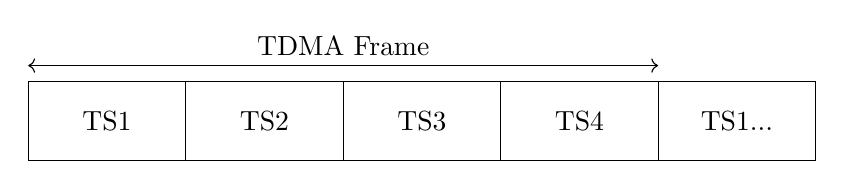
\begin{tikzpicture}
    \draw (0,0) rectangle (2,1) node[pos=0.5] {TS1};
    \draw (2,0) rectangle (4,1) node[pos=0.5] {TS2};
    \draw (4,0) rectangle (6,1) node[pos=0.5] {TS3};
    \draw (6,0) rectangle (8,1) node[pos=0.5] {TS4};
    \draw (8,0) rectangle (10,1) node[pos=0.5] {TS1...};
    
    \draw[<->] (0,1.2) -- (8,1.2) node[midway, above] {TDMA Frame};
\end{tikzpicture}
\end{center}

\begin{mnemonicbox}
\textbf{Mnemonic:} "TIME" - Transmission In Measured Epochs
\end{mnemonicbox}
\end{solutionbox}

\questionmarks{5}{a}{3}
\textbf{Explain T1 carrier system.}

\begin{solutionbox}
\textbf{T1 Carrier System:}

\begin{tabulary}{\linewidth}{L L}
\hline
\textbf{Characteristic} & \textbf{Specification} \\
\hline
\textbf{Data Rate} & 1.544 Mbps \\
\textbf{Channels} & 24 voice channels \\
\textbf{Voice Sampling} & 8000 samples/second \\
\textbf{Sample Size} & 8 bits per sample \\
\textbf{Frame Size} & 193 bits ($24\times8 + 1$) \\
\textbf{Frame Rate} & 8000 frames/second \\
\hline
\end{tabulary}

\textbf{T1 Frame Structure:}

\begin{center}
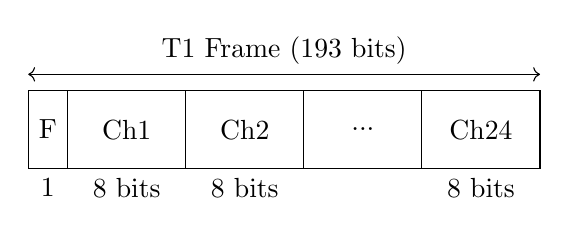
\begin{tikzpicture}
    \draw (0,0) rectangle (0.5,1) node[pos=0.5] {F};
    \draw (0.5,0) rectangle (2,1) node[pos=0.5] {Ch1};
    \draw (2,0) rectangle (3.5,1) node[pos=0.5] {Ch2};
    \draw (3.5,0) rectangle (5,1) node[pos=0.5] {...};
    \draw (5,0) rectangle (6.5,1) node[pos=0.5] {Ch24};
    
    \node[below] at (0.25,0) {1};
    \node[below] at (1.25,0) {8 bits};
    \node[below] at (2.75,0) {8 bits};
    \node[below] at (5.75,0) {8 bits};
    
    \draw[<->] (0,1.2) -- (6.5,1.2) node[midway, above] {T1 Frame (193 bits)};
\end{tikzpicture}
\end{center}

\begin{mnemonicbox}
\textbf{Mnemonic:} "T1-24-8-8" - T1 has 24 channels, 8 bits, 8kHz
\end{mnemonicbox}
\end{solutionbox}

\questionmarks{5}{b}{4}
\textbf{Explain Time Division Multiplexing technique (TDM) in detail.}

\begin{solutionbox}
\textbf{Time Division Multiplexing (TDM):}

\begin{center}
\begin{tikzpicture}[node distance=2cm, auto]
    \node [gtu block] (mux) {Multiplexer};
    \node [gtu block, left of=mux, yshift=1.5cm, xshift=-2cm] (s1) {Signal 1};
    \node [gtu block, left of=mux, yshift=0.5cm, xshift=-2cm] (s2) {Signal 2};
    \node [gtu block, left of=mux, yshift=-0.5cm, xshift=-2cm] (s3) {Signal 3};
    \node [gtu block, left of=mux, yshift=-1.5cm, xshift=-2cm] (s4) {Signal 4};

    \node [gtu block, right of=mux, node distance=3cm] (chan) {Channel};
    \node [gtu block, right of=chan, node distance=3cm] (demux) {Demultiplexer};

    \node [gtu block, right of=demux, yshift=1.5cm, xshift=2cm] (o1) {Signal 1};
    \node [gtu block, right of=demux, yshift=0.5cm, xshift=2cm] (o2) {Signal 2};
    \node [gtu block, right of=demux, yshift=-0.5cm, xshift=2cm] (o3) {Signal 3};
    \node [gtu block, right of=demux, yshift=-1.5cm, xshift=2cm] (o4) {Signal 4};

    \path [gtu arrow] (s1) -- (mux);
    \path [gtu arrow] (s2) -- (mux);
    \path [gtu arrow] (s3) -- (mux);
    \path [gtu arrow] (s4) -- (mux);
    \path [gtu arrow] (mux) -- (chan);
    \path [gtu arrow] (chan) -- (demux);
    \path [gtu arrow] (demux) -- (o1);
    \path [gtu arrow] (demux) -- (o2);
    \path [gtu arrow] (demux) -- (o3);
    \path [gtu arrow] (demux) -- (o4);
\end{tikzpicture}
\end{center}

\textbf{Table of TDM Characteristics:}

\begin{tabulary}{\linewidth}{L L}
\hline
\textbf{Feature} & \textbf{Description} \\
\hline
\textbf{Principle} & Multiple signals share a single channel by taking turns \\
\textbf{Time Allocation} & Each signal assigned a fixed time slot \\
\textbf{Synchronization} & Precise timing required between multiplexer and demultiplexer \\
\textbf{Interleaving} & Samples from different sources interleaved in time \\
\textbf{Types} & Synchronous TDM and Asynchronous (Statistical) TDM \\
\hline
\end{tabulary}

\textbf{TDM Frame Structure:}

\begin{center}
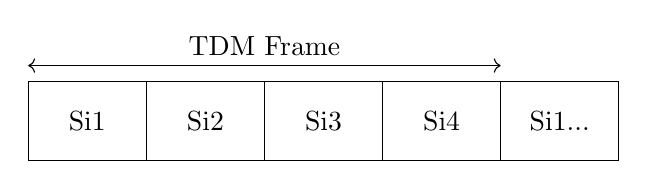
\begin{tikzpicture}
    \draw (0,0) rectangle (1.5,1) node[pos=0.5] {Si1};
    \draw (1.5,0) rectangle (3,1) node[pos=0.5] {Si2};
    \draw (3,0) rectangle (4.5,1) node[pos=0.5] {Si3};
    \draw (4.5,0) rectangle (6,1) node[pos=0.5] {Si4};
    \draw (6,0) rectangle (7.5,1) node[pos=0.5] {Si1...};
    
    \draw[<->] (0,1.2) -- (6,1.2) node[midway, above] {TDM Frame};
\end{tikzpicture}
\end{center}

\begin{mnemonicbox}
\textbf{Mnemonic:} "TWIST" - Time Windows Interleaving Signals Together
\end{mnemonicbox}
\end{solutionbox}

\questionmarks{5}{c}{7}
\textbf{Explain security components of information security in detail.}

\begin{solutionbox}
\textbf{Information Security Components:}

\begin{center}
\begin{tikzpicture}[node distance=2cm, auto]
    \node [gtu block] (sec) {Information Security};
    \node [gtu block, below left of=sec, node distance=3cm] (conf) {Confidentiality};
    \node [gtu block, below of=sec, node distance=2.5cm] (int) {Integrity};
    \node [gtu block, below right of=sec, node distance=3cm] (avail) {Availability};
    
    \node [gtu block, below of=conf, node distance=2cm] (crypt) {Encryption\\Access Control};
    \node [gtu block, below of=int, node distance=2cm] (hash) {Digital Signatures\\Hashing};
    \node [gtu block, below of=avail, node distance=2cm] (backup) {Redundancy\\Backups};

    \path [gtu arrow] (sec) -- (conf);
    \path [gtu arrow] (sec) -- (int);
    \path [gtu arrow] (sec) -- (avail);
    \path [gtu arrow] (conf) -- (crypt);
    \path [gtu arrow] (int) -- (hash);
    \path [gtu arrow] (avail) -- (backup);
\end{tikzpicture}
\end{center}

\textbf{Table of Security Components:}

\begin{tabulary}{\linewidth}{L L L}
\hline
\textbf{Component} & \textbf{Description} & \textbf{Implementation Methods} \\
\hline
\textbf{Confidentiality} & Ensuring information is accessible only to authorized users & Encryption, Access control, Authentication \\
\textbf{Integrity} & Maintaining accuracy and consistency of data & Digital signatures, Hashing, Checksums \\
\textbf{Availability} & Ensuring information is accessible when needed & Redundancy, Backup systems, Disaster recovery \\
\textbf{Authentication} & Verifying identity of users & Passwords, Biometrics, Digital certificates \\
\textbf{Non-repudiation} & Preventing denial of sending/receiving information & Digital signatures, Audit trails \\
\hline
\end{tabulary}

\begin{mnemonicbox}
\textbf{Mnemonic:} "CIA" - Confidentiality, Integrity, Availability
\end{mnemonicbox}
\end{solutionbox}

\questionmarks{5}{a}{3}
\textbf{Explain E1 carrier system.}

\begin{solutionbox}
\textbf{E1 Carrier System:}

\begin{tabulary}{\linewidth}{L L}
\hline
\textbf{Characteristic} & \textbf{Specification} \\
\hline
\textbf{Data Rate} & 2.048 Mbps \\
\textbf{Channels} & 32 time slots (30 voice + 2 signaling) \\
\textbf{Voice Sampling} & 8000 samples/second \\
\textbf{Sample Size} & 8 bits per sample \\
\textbf{Frame Size} & 256 bits ($32\times8$) \\
\textbf{Frame Rate} & 8000 frames/second \\
\hline
\end{tabulary}

\textbf{E1 Frame Structure:}

\begin{center}
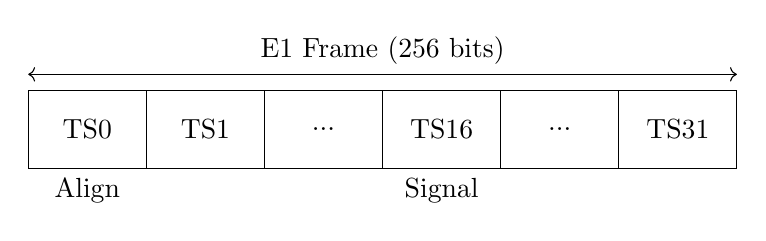
\begin{tikzpicture}
    \draw (0,0) rectangle (1.5,1) node[pos=0.5] {TS0};
    \draw (1.5,0) rectangle (3,1) node[pos=0.5] {TS1};
    \draw (3,0) rectangle (4.5,1) node[pos=0.5] {...};
    \draw (4.5,0) rectangle (6,1) node[pos=0.5] {TS16};
    \draw (6,0) rectangle (7.5,1) node[pos=0.5] {...};
    \draw (7.5,0) rectangle (9,1) node[pos=0.5] {TS31};
    
    \node[below] at (0.75,0) {Align};
    \node[below] at (5.25,0) {Signal};
    
    \draw[<->] (0,1.2) -- (9,1.2) node[midway, above] {E1 Frame (256 bits)};
\end{tikzpicture}
\end{center}

\begin{mnemonicbox}
\textbf{Mnemonic:} "E1-32-8-8" - E1 has 32 channels, 8 bits, 8kHz
\end{mnemonicbox}
\end{solutionbox}

\questionmarks{5}{b}{4}
\textbf{Explain Frequency Division Multiplexing technique (FDM) in detail.}

\begin{solutionbox}
\textbf{Frequency Division Multiplexing (FDM):}

\begin{center}
\begin{tikzpicture}[node distance=2.5cm, auto]
    \node [gtu block] (comb) {Combiner};
    \node [gtu block, left of=comb, yshift=1.5cm, xshift=-2cm] (m1) {Modulator $f_1$};
    \node [gtu block, left of=comb, yshift=0.5cm, xshift=-2cm] (m2) {Modulator $f_2$};
    \node [gtu block, left of=comb, yshift=-0.5cm, xshift=-2cm] (m3) {Modulator $f_3$};
    
    \node [left of=m1, node distance=2cm] {Signal 1};
    \node [left of=m2, node distance=2cm] {Signal 2};
    \node [left of=m3, node distance=2cm] {Signal 3};

    \node [gtu block, right of=comb, node distance=3cm] (chan) {Channel};
    \node [gtu block, right of=chan, node distance=3cm] (filt) {Filters};

    \node [gtu block, right of=filt, yshift=1.5cm, xshift=2cm] (d1) {Demodulator $f_1$};
    \node [gtu block, right of=filt, yshift=0.5cm, xshift=2cm] (d2) {Demodulator $f_2$};
    \node [gtu block, right of=filt, yshift=-0.5cm, xshift=2cm] (d3) {Demodulator $f_3$};

    \path [gtu arrow] (m1) -- (comb);
    \path [gtu arrow] (m2) -- (comb);
    \path [gtu arrow] (m3) -- (comb);
    \path [gtu arrow] (comb) -- (chan);
    \path [gtu arrow] (chan) -- (filt);
    \path [gtu arrow] (filt) -- (d1);
    \path [gtu arrow] (filt) -- (d2);
    \path [gtu arrow] (filt) -- (d3);
\end{tikzpicture}
\end{center}

\textbf{FDM Spectrum:}

\begin{center}
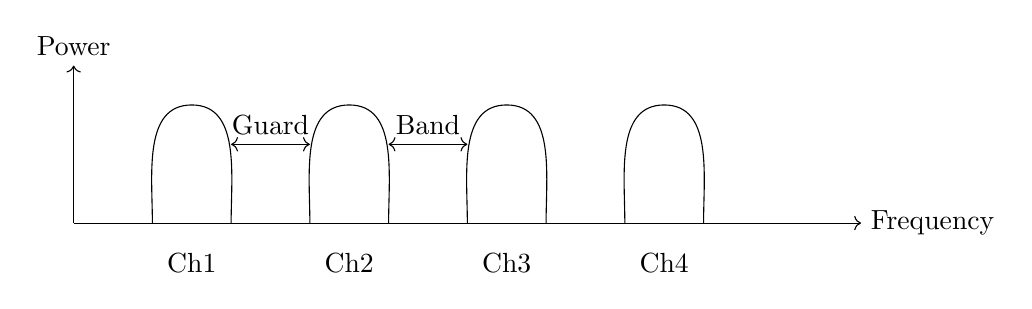
\begin{tikzpicture}
    \draw[->] (0,0) -- (10,0) node[right] {Frequency};
    \draw[->] (0,0) -- (0,2) node[above] {Power};
    
    \draw (1,0) to[out=90,in=180] (1.5,1.5) to[out=0,in=90] (2,0);
    \draw (3,0) to[out=90,in=180] (3.5,1.5) to[out=0,in=90] (4,0);
    \draw (5,0) to[out=90,in=180] (5.5,1.5) to[out=0,in=90] (6,0);
    \draw (7,0) to[out=90,in=180] (7.5,1.5) to[out=0,in=90] (8,0);
    
    \node at (1.5, -0.5) {Ch1};
    \node at (3.5, -0.5) {Ch2};
    \node at (5.5, -0.5) {Ch3};
    \node at (7.5, -0.5) {Ch4};
    
    \draw[<->] (2,1) -- (3,1) node[midway, above] {Guard};
    \draw[<->] (4,1) -- (5,1) node[midway, above] {Band};
\end{tikzpicture}
\end{center}

\begin{mnemonicbox}
\textbf{Mnemonic:} "FROG" - FRequencies Organized with Gaps
\end{mnemonicbox}
\end{solutionbox}

\questionmarks{5}{c}{7}
\textbf{Explain concept and key features of Internet of Things (IoT).}

\begin{solutionbox}
\textbf{Internet of Things (IoT) Concept:}

\begin{center}
\begin{tikzpicture}[node distance=2.5cm, auto]
    \node [gtu block, circle, text width=2cm] (iot) {Internet of\\Things};
    
    \node [gtu block, above of=iot] (data) {Data Collection\\(Sensors)};
    \node [gtu block, right of=iot] (proc) {Analytics\\(AI/ML)};
    \node [gtu block, below of=iot] (act) {Action\\(Actuators)};
    \node [gtu block, left of=iot] (conn) {Connectivity\\(Cloud)};
    
    \path [gtu arrow] (iot) -- (data);
    \path [gtu arrow] (iot) -- (proc);
    \path [gtu arrow] (iot) -- (act);
    \path [gtu arrow] (iot) -- (conn);
\end{tikzpicture}
\end{center}

\textbf{IoT Architecture Layers:}

\begin{center}
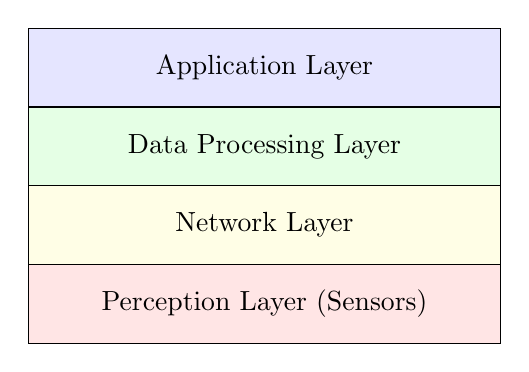
\begin{tikzpicture}
    \draw[fill=blue!10] (0,4) rectangle (6,5) node[midway] {Application Layer};
    \draw[fill=green!10] (0,3) rectangle (6,4) node[midway] {Data Processing Layer};
    \draw[fill=yellow!10] (0,2) rectangle (6,3) node[midway] {Network Layer};
    \draw[fill=red!10] (0,1) rectangle (6,2) node[midway] {Perception Layer (Sensors)};
\end{tikzpicture}
\end{center}

\textbf{Table of IoT Key Features:}

\begin{tabulary}{\linewidth}{L L}
\hline
\textbf{Feature} & \textbf{Description} \\
\hline
\textbf{Connectivity} & Devices connected to internet and each other \\
\textbf{Intelligence} & Smart processing, decision-making capabilities \\
\textbf{Sensing} & Gathering data from environment through sensors \\
\textbf{Expressing} & Taking actions through actuators \\
\textbf{Energy Efficiency} & Low power consumption for battery-operated devices \\
\textbf{Security} & Protection against unauthorized access and attacks \\
\textbf{Scalability} & Ability to add more devices to the network \\
\hline
\end{tabulary}

\begin{mnemonicbox}
\textbf{Mnemonic:} "CASED" - Connected, Automated, Sensing, Expressing, Data-driven
\end{mnemonicbox}
\end{solutionbox}

\end{document}
